先行研究\cite{mura}では雨粒の時間間隔の分布をヒストグラムで表したが近似式を求められていない.
したがって,先行研究\cite{mura}のヒストグラムをガンマ分布を用い近似を行った.

\section{ガンマ分布}
ガンマ分布の定義と性質を以下に示す.chatgpt\cite{gpt}で作成した文書を基に作成している.
ガンマ分布は連続確率分布の一種であり,形状パラメータ \( k > 0 \) と尺度パラメータ \( \theta > 0 \) によって定義される.確率密度関数 (PDF) は以下の式で表せる:

\begin{equation}
f(x; k, \theta) = \frac{x^{k-1} e^{-x/\theta}}{\Gamma(k) \theta^k}, \quad x > 0,
\end{equation}

ここで,\(\Gamma(k)\) はガンマ関数と呼ばれ,次式で定義される:

\begin{equation}
\Gamma(k) = \int_{0}^{\infty} t^{k-1} e^{-t} \, dt.
\end{equation}

ガンマ分布は形状パラメータ \( k \) によって分布の形状が変わり,尺度パラメータ \(\theta\) によってスケールが調整される.

\subsection{基本的性質}
ガンマ分布の平均と分散は以下のように表せる:
\vspace{3zh}
\begin{itemize}
    \item 平均:\(\mathbb{E}[X] = k \theta\)
    \item 分散:\(\mathrm{Var}(X) = k \theta^2\)
\end{itemize}

\vspace{10zh}
\section{検出された雨粒の時間間隔の分布}
取得した降水量2〜13mm/hの取得データをガンマ分布で近似した例を\figref{Fig:5.1}〜\figref{Fig:5.6}に示す.
下記の図はx軸が降水量,y軸が対応する確率密度を表している.
先行研究同様,降水量が少ないほどデータ数が減少していく傾向であった.
形状パラメータは降水量による関連性は見られなかった.このことから,降水量によって分布の形状は変化しない可能性があると考えられる.
一方,尺度パラメータは降水量が増えるほど減少していく傾向が見られた.このことから,降水量が増えるほどデータのばらつきが小さくなる傾向があると考えられる.
\vspace{7.0zh}

\begin{figure}[H]
    \centering
    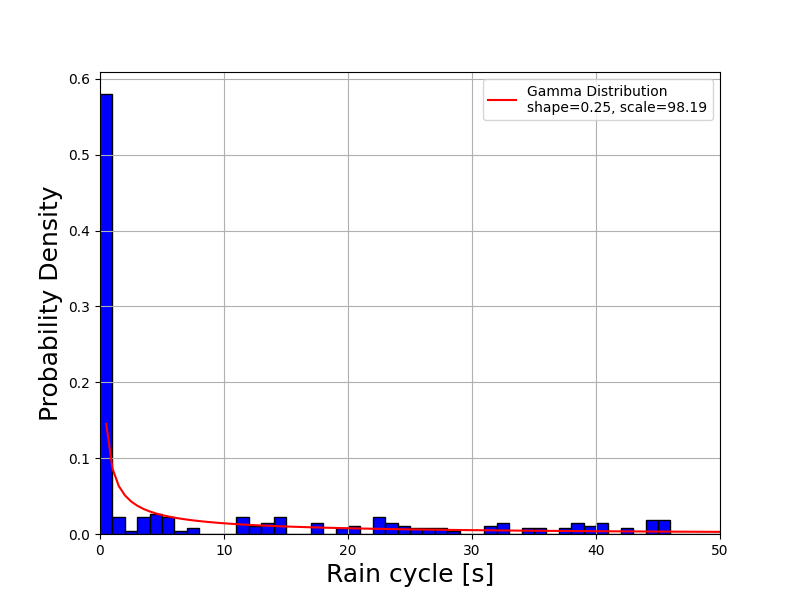
\includegraphics[keepaspectratio, scale=0.5]{images/png/3mm.png}
    \caption{Time interval distribution of detected raindrops (2mm/h)}
    \label{Fig:5.1}
\end{figure}

\begin{figure}[H]
    \centering
    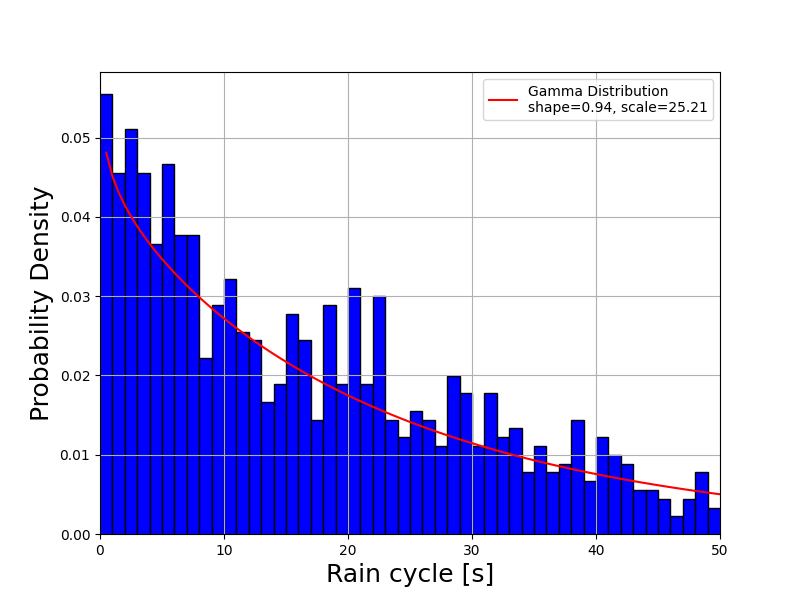
\includegraphics[keepaspectratio, scale=0.5]{images/png/4mm.png}
    \caption{Time interval distribution of detected raindrops (4mm/h)}
    \label{Fig:5.2}
\end{figure}

\begin{figure}[H]
    \centering
    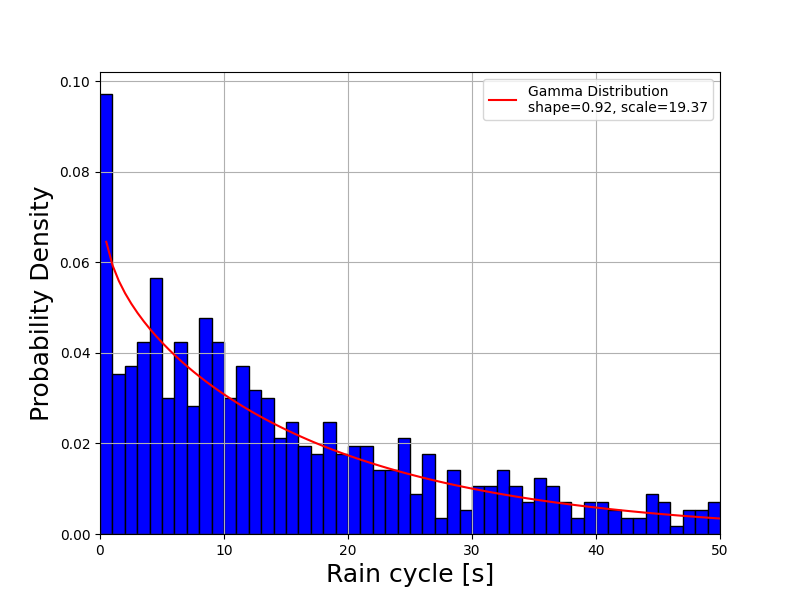
\includegraphics[keepaspectratio, scale=0.5]{images/png/6mm.png}
    \caption{Time interval distribution of detected raindrops (6mm/h)}
    \label{Fig:5.3}
\end{figure}

\begin{figure}[H]
    \centering
    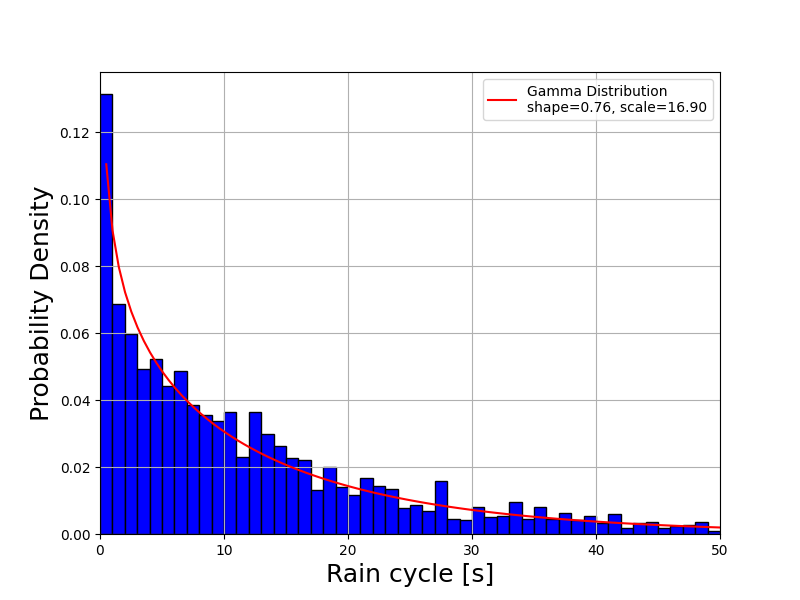
\includegraphics[keepaspectratio, scale=0.5]{images/png/8mm.png}
    \caption{Time interval distribution of detected raindrops (8mm/h)}
    \label{Fig:5.4}
\end{figure}

\begin{figure}[H]
    \centering
    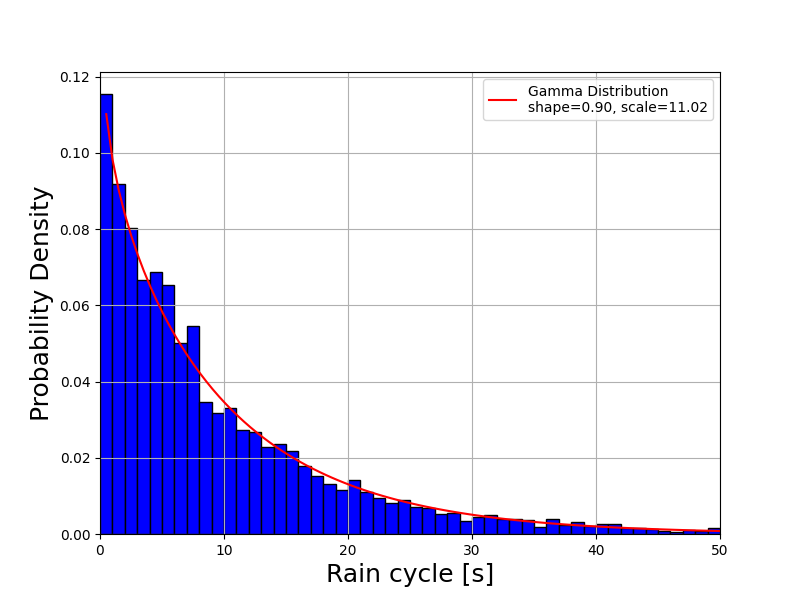
\includegraphics[keepaspectratio, scale=0.5]{images/png/10mm.png}
    \caption{Time interval distribution of detected raindrops (10mm/h)}
    \label{Fig:5.5}
\end{figure}

\begin{figure}[H]
    \centering
    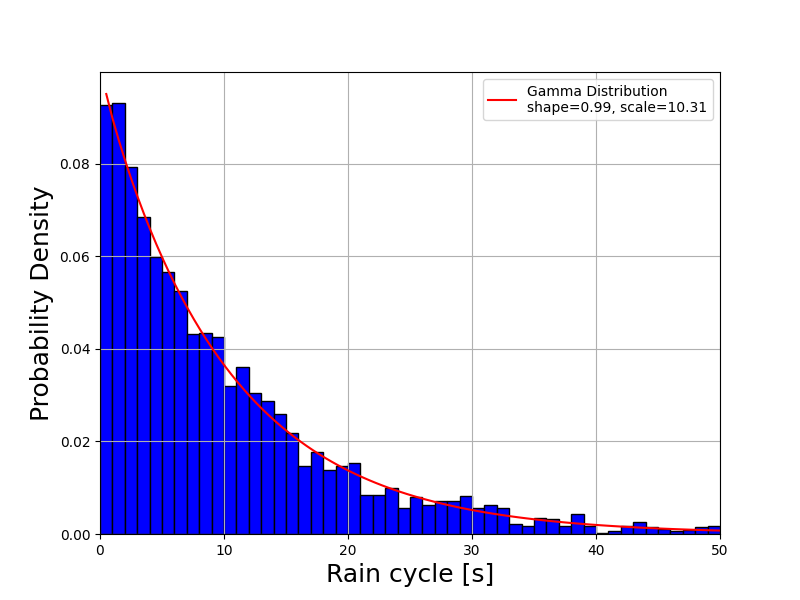
\includegraphics[keepaspectratio, scale=0.5]{images/png/13mm.png}
    \caption{Time interval distribution of detected raindrops (13mm/h)}
    \label{Fig:5.6}
\end{figure}

\section{モデル化}
前節で得た様々な降水量のガンマ分布の近似を基にモデル化を行った.
平均値と降水量の関係を\figref{Fig:5.7}に示す.
また,標準偏差と降水量の関係を\figref{Fig:5.8}に示す.
降水量が増えるほど平均値,標準偏差共に減少していく傾向があることが分かった.
このことから,降水量が増えるほど雨粒の時間間隔が短くなり,ばらつきが小さくなると考えられる.


\begin{figure}[H]
    \centering
    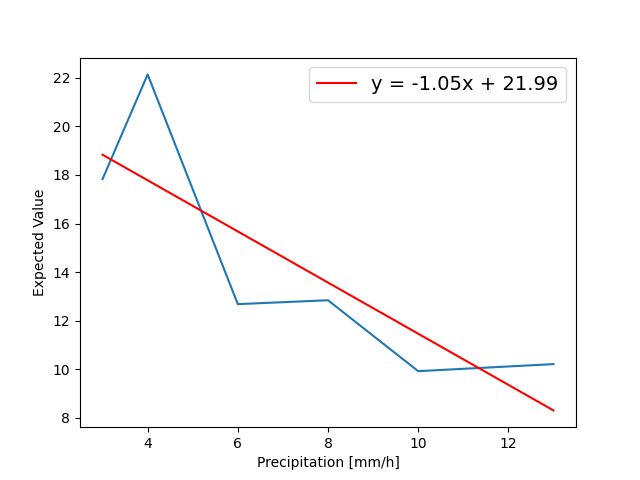
\includegraphics[keepaspectratio, scale=0.5]{images/png/kitaiti.png}
    \caption{Average value of the time interval distribution of detected raindrops}
    \label{Fig:5.7}
\end{figure}

\begin{figure}[H]
    \centering
    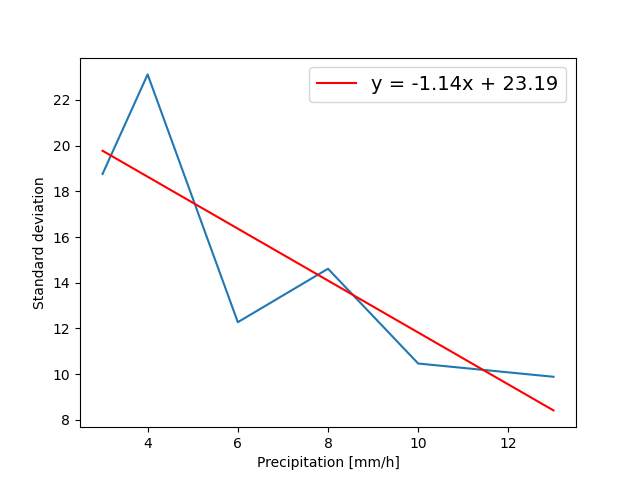
\includegraphics[keepaspectratio, scale=0.5]{images/png/hyouzunhensa.png}
    \caption{Standard deviation of the time interval distribution of detected raindrops}
    \label{Fig:5.8}
\end{figure}